\documentclass[12pt]{article}

%%%%%%%%%%%%%%%%%%%%%%% Don't change anything in here. This space is called the preamble, it is where you tell the computer to load the proper LaTeX packages to perform the math and formatting desired. 
\usepackage{url}
\usepackage{multicol}
\usepackage{amsmath}
\usepackage{esint}
\usepackage{physics} 
\usepackage{siunitx}
\usepackage{bigints}
\usepackage{amsfonts}
\usepackage{textcomp}
\usepackage{xcolor}
\usepackage{tikz}
\usepackage{verbatim}
\usetikzlibrary{calc}
\usetikzlibrary{decorations.pathmorphing}
\usepackage{amsmath,amssymb}
\usepackage{siunitx} 
\usepackage{subcaption} 
\usepackage{blindtext} 
\usepackage{enumerate} 
\usepackage{pgfplots}
\usepackage{graphicx}
\usepackage{dsfont}
\usepackage{float}
\bibliographystyle{iopart-num}
\usepackage{cite}
\usepackage{wrapfig} %preámbulo
\usepackage{enumitem}
\usepackage{pgfplotstable}
\usepackage[compact]{titlesec}  
\usepackage[document]{ragged2e}
\usepackage{tikz,pgfplots}
\usepackage[spanish]{babel}
\usepackage[utf8]{inputenc}
\usepackage{hyperref}
\usepackage{amsmath, amsthm, amssymb}  %I added this so that you can use the align tool for equations!
\usepackage{colortbl}
\usepackage{mathtools}
\usepackage{sectsty}
\usepackage{esint}
\usepackage[makeroom]{cancel}
\usepackage{pgfplots}
\usepackage{graphicx}
\usepackage{dsfont}
\usepackage{float}
\usepackage{pdfpages}
\bibliographystyle{iopart-num}
\usepackage{cite}
\usepackage{wrapfig} %preámbulo
\usepackage{enumitem}
\usepackage{pgfplotstable}
\usepackage[compact]{titlesec}  
\usepackage[document]{ragged2e}
\usepackage{tikz,pgfplots}
\usepackage[spanish]{babel}
\usepackage[utf8]{inputenc}
\usepackage{hyperref}
\newtheorem{thm}{Teorema}[subsection]
\newtheorem{teo}[thm]{Teorema}
\newtheorem{obss}{Obs}[subsection]
\newtheorem{defff}{Def}[subsection]
\newtheorem{conjeture}{Conj}[subsection]
\newtheorem{defn}[defff]{Definición}
\newtheorem{lem}{Lemma}[thm]
\newtheorem{cor}{Corollary}[thm]
\newtheorem{prop}{Proposition}[thm]
\newtheorem{rem}{Remark}[thm]
\newtheorem{ill}{Illustration}[thm]
\newtheorem{conj}[conjeture]{Conjetura}
\newtheorem{obs}[obss]{Observación}
\usepackage{amsmath, amsthm, amssymb}  %I added this so that you can use the align tool for equations!
\usepackage{geometry}
 \geometry{
 a4paper,
 total={170mm,257mm},
 left=20mm,
 top=20mm,
 }
\pgfplotsset{compat=1.14}
\graphicspath{ {images/} }
%%%%%%%%%%%%%%%%%%%%%%%%% Again, Don't change anything Above %%%%%%%%%%%%%%%%%%%%

\newcommand{\eq}[1]{\[#1\]}
\renewcommand{\H}{\mathcal{H}}
\renewcommand{\L}{\mathcal{L}}
\newcommand{\s}[1]{\section{#1}}
\newcommand{\en}[1]{\[\boxed{#1}\]}
\newcommand{\e}[1]{\mathrm{e}^{\qty(#1)}}
\newcommand{\coss}[1]{\cos{\qty(#1)}}
\newcommand{\mc}[1]{\mathcal{#1}}
\newcommand{\md}[1]{\mathds{#1}}
\newcommand{\sinn}[1]{\sin{\qty(#1)}}
\newcommand{\lnn}[1]{\ln{\qty(#1)}}
\newcommand{\inv}[1]{\frac{1}{(#1)}}
\newcommand{\intt}[2]{\int\limits_{#1}^{#2}}
\newcommand{\ointt}[2]{\oint\limits_{#1}^{#2}}
\newcommand{\sumn}[1]{\sum_{#1 =1}^{n}}
\newcommand{\summ}[2]{\sum_{#1 =1}^{#2}}
\newcommand{\pp}[2]{\vec{#1}\cdot\vec{#2}}
\newcommand{\pc}[2]{\vec{#1}\, \cross\, \vec{#2}}
\newcommand{\eva}[3]{\eval{#1}_{#2}^{#3}}
\renewcommand{\ss}[1]{\subsection{#1}}
\newcommand{\sss}[1]{\subsubsection{#1}}
\newcommand{\xn}[1]{{#1}_{1},{#1}_{2},\cdots,{#1}_{n}}
\newcommand{\so}{\[\textrm{\textbf{Solución}} \]}
\newcommand{\ej}{\[\textrm{\textbf{Ejemplo}} \]}
\newcommand{\vl}{\,\,\, \vline \,\,\,}
\newcommand{\hl}{\\ \hrulefill \\}
\newcommand{\ob}{ \textit{\textbf{Observación:}} \\}
\newcommand{\pua}{$\bullet \, $}
\newcommand{\eqreff}[1]{Ecuación [\ref{#1}]}
\newcommand{\fgref}[1]{Figura [\ref{#1}]}

%%%%%%%%%%%%%%%%%%%%%%%%%%%%%%5
% Creación de colores
\definecolor{rojo}{RGB}{255, 0, 0}
\definecolor{negro}{RGB}{0, 0, 0}
\definecolor{burdeo}{RGB}{231, 76, 60}
\definecolor{fucsia}{RGB}{255, 0, 171}
\definecolor{morado}{RGB}{142, 69, 212}
\definecolor{verde}{RGB}{26, 139, 73}
\definecolor{violeta}{RGB}{155, 89, 182}
\definecolor{celeste}{RGB}{0, 176, 255}
\definecolor{azul}{RGB}{18, 3, 119}
\definecolor{azul_fosfo}{RGB}{10, 0, 255}

%%%%%%%%%%%%%%
%Colores%
\newcommand{\rojo}[1]{{\color{rojo}#1}}
\newcommand{\negro}[1]{{\color{negro}#1}}
\newcommand{\azul}[1]{{\color{azul}#1}}
\newcommand{\verde}[1]{{\color{verde}#1}}
\newcommand{\burdeo}[1]{{\color{burdeo}#1}}
\newcommand{\rosa}[1]{{\color{fucsia}#1}}
\newcommand{\morado}[1]{{\color{morado}#1}}
\newcommand{\violeta}[1]{{\color{violeta}#1}}
\newcommand{\celeste}[1]{{\color{celeste}#1}}
\newcommand{\azulf}[1]{{\color{azul_fosfo}#1}}
%%%%%%%%%%%%%%%%%%%%%%%%%%%%%%%%%%%%%%%
%%%%%%%%%%%%%%%%%%%%%%%%%%%%%%%%%%%%%%%%%

%%Figuras
\begin{comment} %Figura
\begin{figure}[h!]
    \centering
    \includegraphics[width=0.5\textwidth]{}
    \caption{}
    \label{}
\end{figure}
\end{comment}
%Importar PDF
\begin{comment}
 \includepdf[pages=(pagina inicial)-(pagina final)]{direccion de archivo}
\end{comment}
%%Comando para tachar con colores y señalar que se reemplazó
\begin{comment}
 Cancelar con colores ; \Cancel[blue]{2}+\Cancel[red]{1}-
 \Cancel[blue]{2}-\Cancel[red]{1}\\
 
 Cancelar normal; \Cancel{x}\\
 
 Cancelar con una cruz; \xCancel{}\\
 
 Cancelar e indicar con qué valor se reemplazó ; \cancelto{Se vuelve esto}{Reemplaza esto}\\
 Separar la hoja con una raya negra: \hline 
 Separar la hoja con puntos negros: \dotfill
 
\end{comment}
%%%%%%%%%%%%%%%%%%%%%%%%5

% Derivadas
\begin{comment}
 n-esima Derivada Normal (si quieres la normal borra el [n]); \dv[n]{f}{x} \\
 n-esima derivada parcial (si quieres la normal borra el [n]) : \pdv[n]{f}{x}\\
 derivada mixta: \pdv{f}{x}{y}  \\
\end{comment}
%%%%%%%%%%%%%%

%Integral: 
\begin{comment}
 Integral de linea con limites inferior y superior: \oint \oiint \limits_{}^{}
\end{comment}
%%%%%%%%%%%%%




\begin{document}

%%ESTO ES EL ENCABEZADO
\begin{flushleft}
    \begin{figure}[t]
    \raggedright

\includegraphics[scale=0.2]{Logo_UTFSM.png}
    \label{fig:imagen}
\end{figure}
\end{flushleft}

\begin{flushright}
\vspace{-4cm}
\hspace{8cm}
\textbf{Universidad Técnica Federico Santa María\\
\hspace{9cm}Departamento de \textbf{Fisica}\\
\hspace{9cm}FIS210\\
\hspace{9cm}2°. Semestre 2021}
\end{flushright}

\begin{center}
    \large
    %TITULO DEL PAPER%
    \textbf{FIS210: Clase 22 }\\
    \large
    \author[Bastián Castorene$^1$\\
    \today\\
    {$^1$\small{\textit{Estudiante de Licenciatura en Física, Departamento de Física, UTFSM}}}\\
\end{center}
\s{Tipos de Función Generatriz}
\ss{Función Tipo I, q y Q}

$$F= F_1 (q,Q,t)$$
Incluye a q y Q.

$$p_i = \pdv{F_1}{q_i}$$
$$P_i= - \pdv{F_1}{Q_1}$$
$$\mc{H}`= \mc{H} + \pdv{F_1}{t}$$
\ss{Función Tipo II, q y P}
$$F= F_2(q,P,t)$$
Incluye a q y P
$$F_2(q,P,t)= F+\sumn{i}P_iQ_i$$
\begin{align}
dF_2 &= dF + \sumn{i} \qty(P_i dQ_i + Q_i dP_i)=\sumn{i}\qty(p_i dq_i + Q_i dP_i)- \qty(\H -\H')dt\\
\end{align}
\en{p_i= \pdv{F_2}{q_i} \vl Q_i=\pdv{F_2}{P_i} \vl \H' = \H + \pdv{F_2}{t}}

\ss{Función Tipo III, p y Q}
\begin{align}
&F= F_3\qty(p,Q,t)= F - \sumn{i} qip_i
\end{align}

\en{q_i= -\pdv{F_3}{p_i} \vl P_i=-\pdv{F_3}{q_i} \vl \H' = \H + \pdv{F_3}{t}}

\ss{Función Tipo IV, p y P}
Aqui se tendran que hacer dos transformadas de Legendre.

\begin{align}
F= F_4 \qty(p,P,t)= F + \sumn{i}\qty(Q_iPi-q_i p_i)
\end{align}

\en{q_i= -\pdv{F_4}{p_i} \vl Q_i=\pdv{F_4}{P_i} \vl \H' = \H + \pdv{F_4}{t}}

\hrulefill\\
\vspace{3mm}
\rosa{Estas funciones se pueden usar de 2 maneras.\\
\pua Dar una funcion generatriz y eso va a dar una transformacion canonica.\\
\pua Dada una transformacion que creemos que es canonica, nos podemos asegurar que lo es \textbf{si} encontramos su generatriz.\\
Se deben mencionar que existen otros metodos de conocer si es canonica, como por ejemplo con corchetes de poisson. Osea, no es impresindible. Pero a veces ayuda a plantear ciertos parametros.}\\
\vspace{3mm}
\hrulefill
\vspace{3mm}
\ej
\begin{align}
F=F_2\qty(q,P)	= - \frac{P}{q}\\
\implies p= \pdv{F_2}{q}= \frac{P}{q^2}\\
\implies Q= \pdv{F_2}{P}= -\frac{1}{q}
\end{align}
\en{p= - \frac{P}{q^2} \vl Q= -\frac{1}{q}\vl \H' = \H}
\ej
\begin{align}
Q = \lnn{\frac{p}{q}} \vl 	P=-\frac{p}{q}\qty(\frac{q^2}{2}+1)
\end{align}
Buscamos una $F_1(q,Q)$
\begin{align}
&p= q \e{Q} \vl 	p= \pdv{F_1}{q}\\
&\pdv{F_1}{q}= q \e{Q} \implies F_1 = \int q \e{Q} \, dq\\
&F_1= \frac{q^2}{2}\e{Q} + h(Q)\\
&P= - \pdv{F_1}{Q} = - \frac{q^2}{2}\e{Q} + h'(Q)\\
&P=-\frac{p}{q}\qty(\frac{q^2}{2}+1)= -\e{Q} \qty(\frac{q^2}{2}+1)\\
&-\e{Q} \qty(\frac{q^2}{2}+1) =   - \frac{q^2}{2}\e{Q} + h'(Q)\\
&\therefore h'(Q)= \e{Q} \implies h{Q}=\e{Q}
\end{align}
\en{F_1 = - \frac{q^2}{2}\e{Q} + \e{Q} }
En resumen, empezamos con una transformacion, pero como fuimos capaces de encontrar la generatriz automaticamente es canonica.
\ej
\begin{align}
&\frac{p^2}{2m}=J\omega \cos[2](\theta)	\vl \frac{k}{2}q^2 = J \omega \sin[2](\theta)\\
&q,p \rightarrow \theta,J\\
&p=\sqrt{2m\omega J \cos[2](\theta)}\vl q= \sqrt{\frac{2J}{m\omega}} \sin(\theta)\\
&Buscamos\,\, F_1(q,\theta)\\
&p=\pdv{F_1}{q} \bigg/ dividimos\, p\,y\,q\\
&\frac{p}{q}=mv\cot{\theta}\\
&p=qmv \cot{\theta}\bigg/ \int dq\\
&F_1 = \frac{q^2}{2}mv \cot{\theta} + h(\theta)\\
&\pdv{F_1}{\theta}= \frac{q^2}{2}mv \frac{1}{\sin[2](\theta)} + h'(\theta)\\
&\frac{q^2}{2}mv \frac{1}{\sin[2](\theta)} + h'(\theta)= \frac{m\omega}{2 \sin[2](\theta)}q^2 \implies h'(\theta)=0
\end{align}
\en{F_1 = \frac{q^2}{2}mv \cot{\theta}}
\en{Si\, \H = \frac{p^2}{2m}+\omega^2 q^2 \implies \omega J}
Es interesante ver que encontrar la Generatriz para las variables angulos accion y encontrar un metodo para hallarlas.\\
\s{Condiciones Directas para saltarnosla Generatriz}
Derivando las relaciones ya conocidas. \\
\textbf{$F_1$}\\
\begin{align}
\pdv{p_i}{Q_j}= \pdv{Q_j}\qty(\pdv{F_1}{q_i})= \pdv{q_j}\qty(-P_j)=-\pdv{P_j}{q_i} = -\pdv{P_i}{q_i}\\
\end{align}
\en{\pdv{p_i}{Q_j}= -\pdv{P_i}{q_i}}
Todo esto se repite para $F_2,F_3,F_4$ obteniendo lo siguiente
\rojo{\en{\pdv{p_i}{Q_j}= -\pdv{P_j}{q_i} \vl \pdv{p_i}{P_j}= \pdv{Q_j}{q_i}\vl \pdv{q_i}{Q_j}= \pdv{P_j}{p_i} \vl \pdv{q_i}{P_j}= -\pdv{Q_j}{p_i} }}
\begin{equation}
 \label{eq_en}	
\end{equation}

Con estas relaciones bastan y sobran con verificar un par para que la transformacion es canónica sin pasar por la generatriz.\\

\s{Relación de corchetes de Poisson y transformaciones canónicas.}

Esta es la definición del Corchete de Poisson{\footnote{Poisson fue un matemático Francés que estudiaba en la Politecnica cuando Legendre era profesor. Su primer paper fue a los 18 años y fue un matematica prolijo, existen derivadas, integrales y distribuciones estadisticas asociados a él. Y sus famosos corchetes de Poisson.}}.
Estos corchetes seran sumamente util
\begin{align}
[f,g]\equiv \sumn{i} \qty(\pdv{f}{q_i} \pdv{g}{p_i} - \pdv{f}{p_i} \pdv{g}{q_i})	
\end{align}
Corchetes de Poisson elementales:

\begin{align}
	&{[f, g]=-[g, f]} \\
 &{[f, c]=0} \\
&{\left[c_{1} f_{1}+c_{2} f_{2}, g\right]=c_{1}\left[f_{1}, g\right]+c_{2}\left[f_{2}, g\right]} \\
&{\left[f_{1} f_{2}, g\right]=\left[f_{1}, g\right] f_{2}+f_{1}\left[f_{2}, g\right]} \\
&{\left[f, q_{a}\right]=\frac{\partial f}{\partial p_{a}}, \quad\left[f, p_{a}\right]=-\frac{\partial f}{\partial q_{a}}} \\
&{\left[q_{a}, q_{b}\right]=0, \quad\left[p_{a}, p_{b}\right]=0,} \\
&{\left[p_{a}, q_{b}\right]=\delta_{a b},}
\begin{cases}
&1 \,\, si \,\,\,\,i=j\\	
&0\,\, si  \,\,\,\,i \neq j
\end{cases}
\\
&{[[f, g], h]+[[h, f], g]+[[g h], f]=0}
\end{align}
Algunas nociones muy utiles:
\begin{align}
	[Q_i,P_j]_{q,p}= \sumn{i} \qty(\pdv{Q_i}{q_k} \pdv{P_i}{p_k} - \pdv{Q_i}{p_k} \pdv{P_i}{q_k})
\end{align}
Gracias a las ecuaciones de la \eqreff{eq_en} podemos reemplazar en la Ecuacion anterior, porque estas son canonicas:
\begin{align}
		[Q_i,P_j]_{q,p}&= \sumn{i} \qty(\pdv{Q_i}{q_k} \cancelto{\pdv{q_k}{Q_j}}{\pdv{P_i}{p_k}} - \pdv{Q_i}{p_k}\cancelto{- \pdv{p_k}{Q_j}}{ \pdv{P_i}{q_k}})\\
		[Q_i,P_j]_{q,p}&= \sumn{i} \qty(\pdv{Q_i}{q_k} \pdv{q_k}{Q_j} + \pdv{Q_i}{p_k}\pdv{p_k}{Q_j})\\
		&\dv{Q_i}{Q_j}= \delta_{ij} \nonumber
\end{align}
$\therefore$ Esta es otra forma de comprobar si una transformación es canonica.
\rojo{\en{[Q_i,P_j]_{q,p}= \delta_{ij}}}
Existe otra propiedad interesante que relacion las coordenadas originales con las nuevas. Es decir, da lo mismo cuales coordenadas y momentos generalizados uses, darán lo mismo si son canónicas.

\rojo{\en{[f,g]_{q,p}= [f,g]_{Q,p}}}
\s{Transformación canónica Infinitesimal}
Basicamente, llevar el Teorema de Noether a otras perspectivas. Y nos permite una interpretación distinta e interesante.\\
Usaremos una $F_2$ solo para empezar, pueden usar cualquiera.\\
\begin{align}
&F_2(q,P)= \underbrace{\sumn{i} \qty(q_i P_i)}_{\textit{Identidad}} + \epsilon \, G(q,p,t),\,\,\, \epsilon <<1\\	
&p_i = \pdv{F_2}{q_i}= P_i + \epsilon \pdv{G}{q_i}\implies \boxed{P_i=p_i =-\epsilon \, \pdv{G}{q_i}}\\
&Q_i= \pdv{F_2}{P_i}=q_i + \epsilon \, \pdv{G}{P_i}\approx q_i + \epsilon \pdv{G}{p_i}\\
&\pdv{G}{P_i}= \pdv{G}{p_i} + \order{\epsilon}
\end{align}
Estos cuadros resumen que condiciones deben cumplirse para que una. transformación infinitesimal sea canónica.
\rojo{\en{P_i=p_i =-\epsilon \, \pdv{G}{q_i}\vl Q_i= q_i + \epsilon \pdv{G}{p_i}} }
G es la generatriz de la transformacion canonica infinitesimal.
\ss{Evolución Temporal Infinitesimal}
Elegimos 
\begin{align}
G=\H,\,\, \epsilon=dt\\
&Q_i = q_i +dt \underbrace{\pdv{\H}{p_i}}_{\dot{q}_i}\\
&Q_i = q_i + \dot{q}_i dt\bigg/ \textit{Hacemos Taylor a primer orden}\\
&\azul{Q_i(t)= q_i\qty(t+dt)} + \cancel{\order{t^2}}\\
&P_i = p_i - dt \qty(\pdv {\H}{q_i})\\
&P_i = p_i - \dot{p}_i dt
\end{align}
\en{Q_i(t)=q_i \qty(t+dt)\vl P_i(t)= p_i \qty(t+dt)}
La evolución temporal es una transformación canónica generada por el $\H$. Si esto es posible, entonces existe la inversa, que nos lleve del valor en cada tiempo a las condiciones iniciales.\\

\s{Teorema de Liouville}
Liouville demostró una propiedad fundamental del espacio de fases, hace la siguiente afirmación.\\

\begin{figure}[h!]
    \centering
    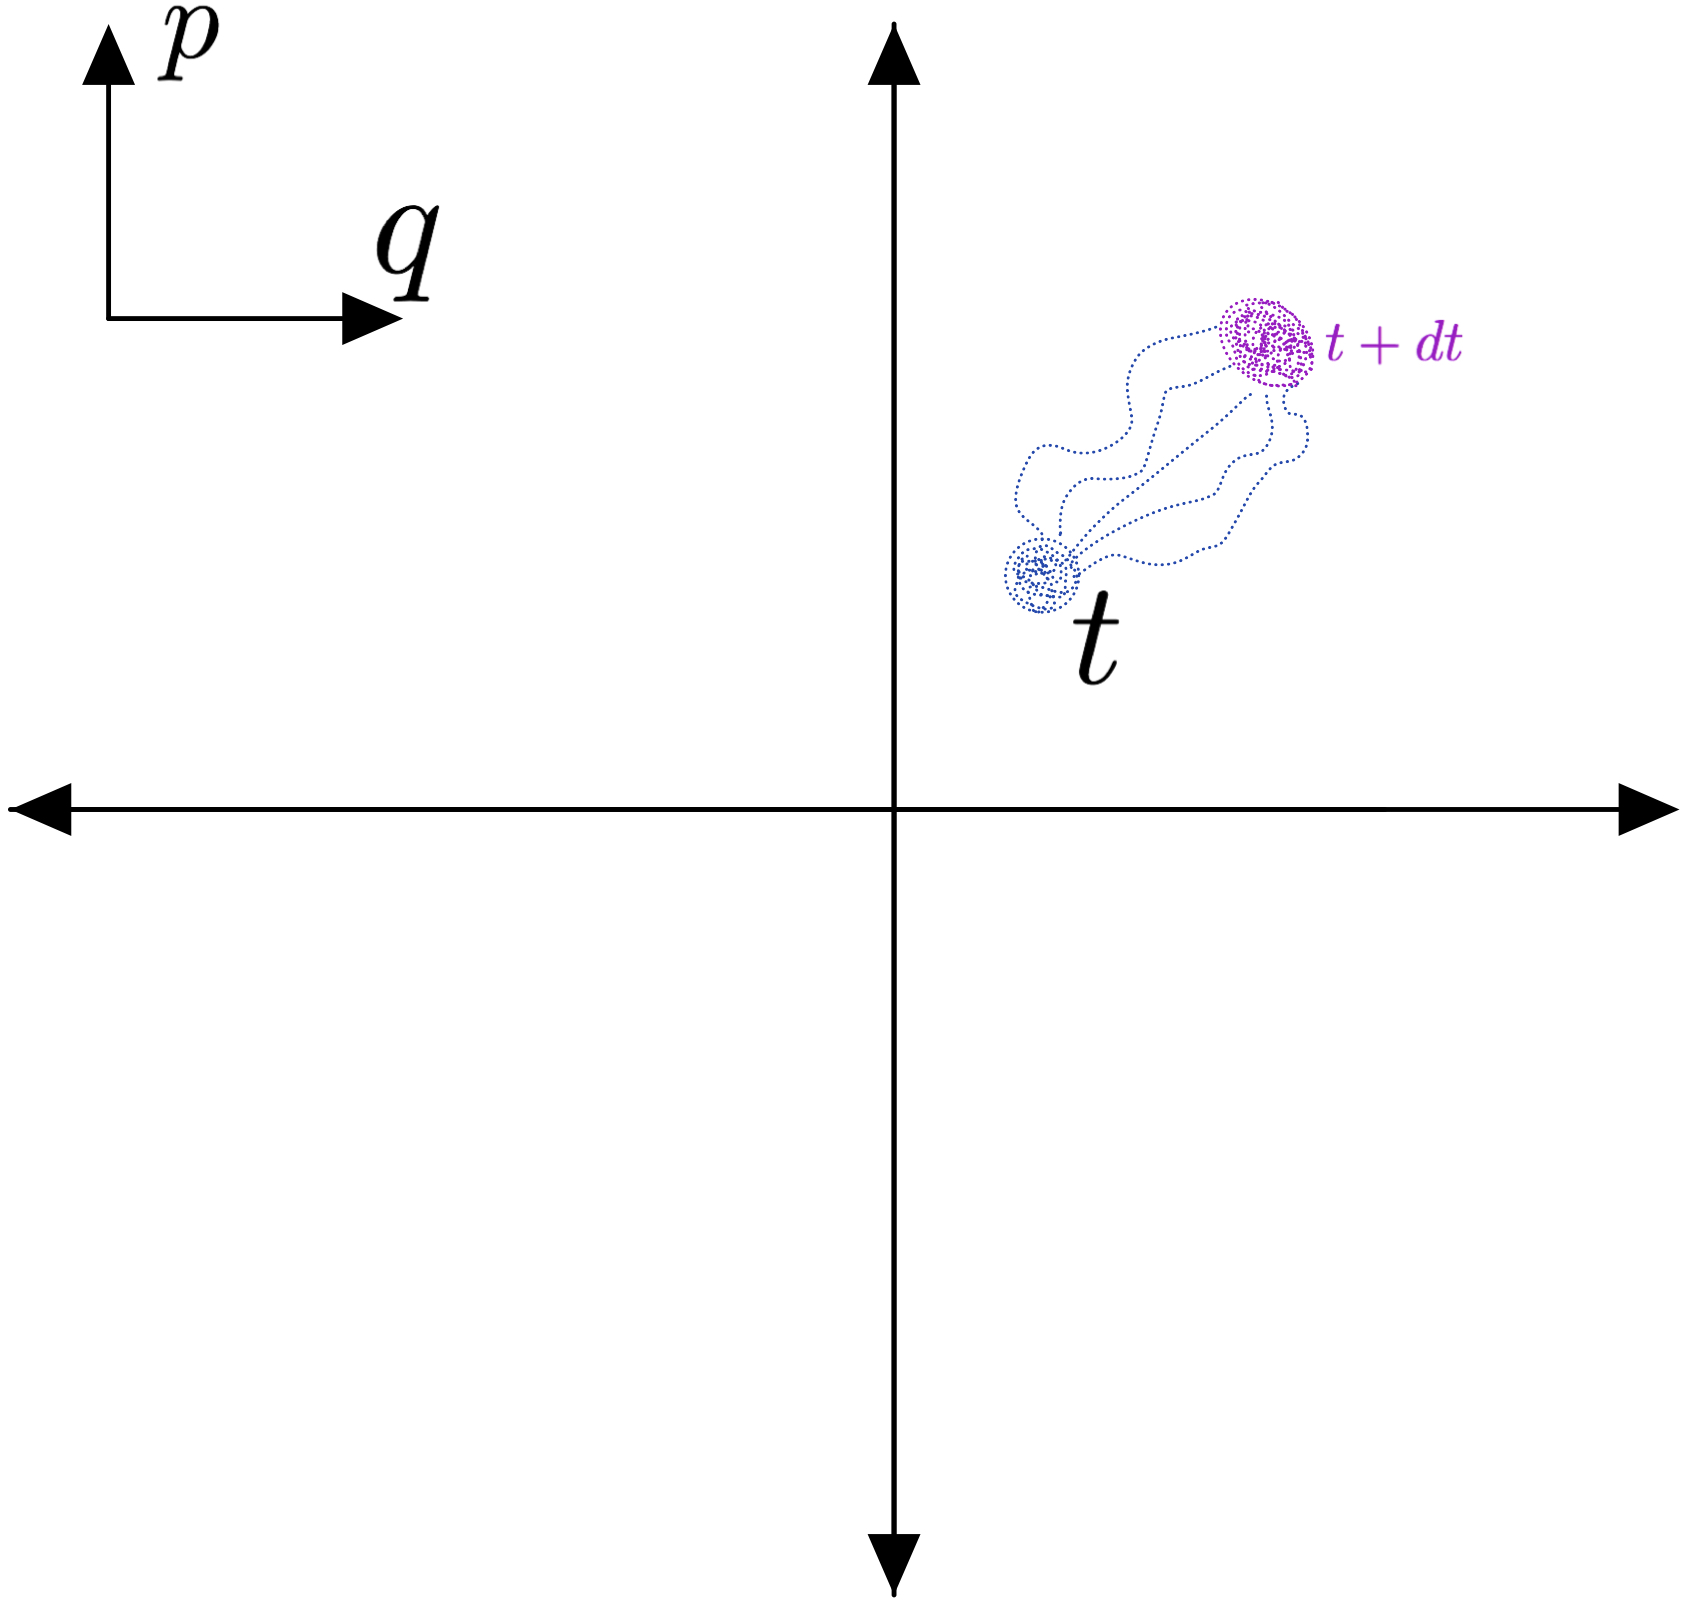
\includegraphics[width=0.5\textwidth]{lou.png}
    \caption{Representación del Teorema de Liouville}
    \label{lou}
\end{figure}

Existe una densidad de estados en el espacio de fases $\rho = \frac{N}{\Gamma}$ es decir, la cantidad de estados iniciales dividido en el volumen en el espacio de fases. Cualquier transformación canónica mantiene el valor del volumen del espacio de fases como muestra la \fgref{lou}. Entonces,  
\teo{La densidad de estados en el espacio de fases se mantiene constante ante la evolución temporal.} 
\ej
\ss{Analogía con un fluido incompresible}
Sea $\vec{u}$ un campo de velocidad,
\begin{align}
&\vec{u}=\qty(\xn{\dot{q}},\xn{\dot{p}})	\\
&\div{\vec{u}}= \qty(\pdv{\dot{q}_1}{q_1}+ \pdv{\dot{q}_2}{q_2}+\cdots+ \pdv{\dot{p}_1}{p_1}+ \pdv{\dot{p}_2}{p_2}+\cdots \pdv{\dot{p}_n}{q_n})\\
&\dot{q_i}=\pdv{\H}{p_i}\vl \dot{p}_i=-\pdv{\H}{q_i}\\
&\div{\vec{u}}= \qty(\pdv{\dot{q}_1}{q_1}+ \pdv{\dot{q}_2}{q_2}+\cdots+ \pdv{\dot{p}_1}{p_1}+ \pdv{\dot{p}_2}{p_2}+\cdots \pdv{\dot{p}_n}{q_n})\\
&\div{\vec{u}}= \qty(\pdv{\H}{q_i}{p_i}+
\cdots-\pdv{\H}{p_i}{q_i}\cdots)\\
&\div{\vec{u}}= \qty(\pdv{\H}{q_i}{p_i}+
\cdots-\pdv{\H}{q_i}{p_i}\cdots)\\
&\div{\vec{u}}=0
\end{align}
Este es el teorema de Liouville que se demuestra mediante el formalismo Hamiltoniano.

\s{Corchetes de Poisson, Leyes del movimiento y de conservación}

\begin{align}
&Sea\, f(q,p,t)\\
&\dv{f}{t}= 	\pdv{\H}{t}+\sumn{i} \qty(\pdv{f}{q_i}\dot{q}_i+\pdv{f}{p_i}\dot{p})\\
&\dv{f}{t}= 	\pdv{\H}{t}+\sumn{i} \qty(\pdv{f}{q_i} \cancelto{\pdv{\H}{p_i}}{\dot{q}_i}+\pdv{f}{p_i} \cancelto{-\pdv{\H}{q_i}}{\dot{p}_i})
\end{align}
\rojo{\en{\dv{f}{t} = \pdv{f}{t}+[f,\H]}}
Esta ecuación es muy importante, porque nos permite escribir de otra forma la formulación Hamiltoniana. Y cualquier función de las variables dinámicas del sistema cumple con esta ecuación.\\
$f$ es constante de movimiento si 
\begin{align}
\dv{f}{t}=0 \implies \pdv{f}{t}= -[f,\H]
\end{align}
 En particular, si la funcion no depende explicitamente del tiempo, entonces:
 \begin{align}
 Si\, \pdv{f}{t}=0,\, f=f(q,p) \implies \boxed{[f,\H]=0}
 \end{align}
Si esto se cumple es constante de movimiento.
\cor{Si $f_1$ y. $f_2$ son constantes de movimiento $\implies$ $[f_1,f_2]$ también es constante de movimiento.}
Esto se demuestra mediante la Identidad de Jacobi. 
\azulf{\en{[f_1,[f_2,f3]]+ [f_2,[f_3,f_1]] +[f_3,[f_1,f_2]]=0}}
\end{document}